\newpage
\subsection{Utiliser RGtk2}

\paragraph{Prérequis} Vous devez avoir une version de R récente déjà présente sur votre ordinateur ; le mieux est de récupérer les sources les plus à jour et de les compiler directement pour votre système. 
\\ \\
Le package RGL se trouve dans la liste des package disponnibles pour R à cet adresse : http://cran.r-project.org/ section "Packages", "sorted by Names", "rgtk". Le fichier à récupérer est le "package source" en tar.tgz. Une fois que ce fichier est téléchargé, lancez une invite de commande R et saisissez : 

\begin{lstlisting}
> install.packages("$HOME/Downloads/RGtk2_2.20.25.tar.gz")
\end{lstlisting}

Le chemin passé en paramètre est un exemple, donnez le chemin vers le fichier que vous avez téléchargé. Celà devrait prendre un peu de temps. \\ \\
Une fois l'installation terminée vous devez linker le package dans l'environnement courrant (et vous devrez le faire à chaque début de session R où vous aurez besoin de RGL) : 

\begin{lstlisting}
> library(RGtk2)
\end{lstlisting}
\newpage

\subsection{Première fen\^etre avec RGtk2}

Voici un code court qui va nous permettre d'afficher une fen\^etre avec le label "hello world". \\

\begin{lstlisting}
>library(RGtk2)
 
createWindow <- function()
{
    window <- gtkWindow()
 
    label <- gtkLabel("Hello World")
    window$add(label)
}
 
>createWindow()
\end{lstlisting}

\begin{center}
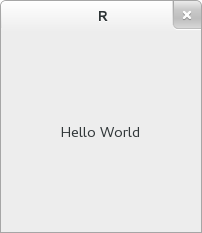
\includegraphics[scale=0.5]{hello.png}\\
\textit{Résultat du code ci-dessus}
\end{center}

Maintenant on va expliquer chacune des lignes de code. La première ligne \textbf{window <- gtkWindow()} nous permet de créer une fen\^etre vide. Ensuite l'appel à la fonction \textbf{gtkLabel()} permet de créer un label qu'il faudra ensuite ajouter à la vue car pour le moment la vue est vide m\^eme si les éléments à ajouter sont déclarés. Enfin gr\^ace à la dernière ligne, \textbf{window\$add(label)} on ajoute le label à la vue. \\

\subsection{Quelques fen\^etres utiles}

\subsubsection{Une fen\^etre en plein écran}
Pour afficher une fen\^etre en plein écran, il faut créer la vue et ensuite lui demander de passer en plein écran. 

\begin{lstlisting}
> win <- gtkWindow()
> gtkWindowFullscreen(win)
\end{lstlisting}

La fonction \textbf{gtkWindowFullscreen(win)} prend en paramètre un objet de type gtkWindow. 

\subsubsection{Des onglets dans la vue}
Une fen\^etre avec des onglets est une chose intéressante à avoir pour l'interface utilisateur. 

\begin{lstlisting}
> window.master <- gtkWindow("toplevel",show=FALSE)
> 
> forms.notebook <- gtkNotebook()
> forms.notebook$setTabPos("top")
> 
> form1.notebook <- gtkNotebook()
> form1.notebook$setTabPos("top")
> 
> form1.boxp1.y3 <- gtkVBox(FALSE,3)
> form1.boxp2.ud <- gtkVBox(FALSE,2)
> forms.notebook$add(form1.notebook)
> window.master$add(forms.notebook)
> 
> window.master$show()

\end{lstlisting}

\begin{itemize}
\item \textbf{gtkNotebook} est une conteneur de vue avec des onglets. \\
\item \textbf{form1.boxp1.y3 <- gtkVBox(FALSE,3)} permet de créer une gtkVBox qui sera notre premier onglet. \\
\item \textbf{forms.notebook\$add(form1.notebook)} : on ajoute le formulaire form1 au formulaire principal forms qui sera ensuite ajouté à la vue via la commande \textbf{window.master\$add(forms.notebook)}. \\
\item \textbf{window.master\$show()} affiche la fenêtre complète. L'appel de cette fonction est obligatoire car on avait choisi de ne pas afficher la fenêtre lors de sa création. 
\end{itemize}

\subsection{La gestion des événements}
La gestion des événements dans rgtk2 n'est pas beaucoup documenter. Mais les fonctions pour les gérer existent dns le package. 




